\chapter{Estudo do estado da arte}
\label{chap:sota}

\section{Robôs Antropormóficos}
\label{ssec:robos}

Robôs antropormóficos, também conhecidos como humanoides, possuem uma estrutura baseada no corpo humano, com  membros e movimentos que visam uma mobilidade que permita ao robô realizar tarefas diversificadas, principalmente para auxiliar as pessoas em atividades diárias, para o entretenimento e realizar tarefas de risco.

De acordo com \citeonline{Li20211} em comparação com outros tipos de robôs, os humanoides são mais adaptáveis ao ambiente e possuem uma boa habilidade para evitar obstáculos, por isso atraem a atenção de muitos pesquisadores.

Estes robôs movimentam-se e ajustam o seu equilíbrio por meio das suas duas pernas, inclusive em terrenos irregulares. Sendo a habilidade de andar com um bom equilíbrio a sua habilidade mais básica.

Para ter uma boa mobilidade e ser capaz de realizar as tarefas propostas o robô deve possuir uma locomoção rápida e estável, por isso o gerador de trajetórias e o controlador são projetados visando uma locomoção rápida, flexível e robusta. Portanto, são estes os principais desafios no desenvolvimento deste tipo de robô.


%/todo: inserir as outras referencias

\subsection{Definição}
\label{ssec:defi}

Os robôs antropormóficos, também conhecidos como humanoides, são robôs que possuem atributos semelhantes a forma humana como cabeça, braços e pernas. São robôs bípedes, ou seja, que se locomovem sobre os dois pés.

\subsection{Componentes principais}
\label{ssec:comp}

A percepção visual é fundamental para a maioria dos sistemas autônomos que operam em ambientes repletos de obstáculos e para realizar uma série de tarefas essenciais como interagir com o humano, manipular e rastrear objetos. \cite{Joseph2018} 

\citeonline{Chatterjee2017603} aponta que os robôs domésticos utilizam da Inteligência Artificial para possuir habilidades como reconhecimento de voz, reconhecimento facial humano, emoção, entre outros.

E, para garantir que o robô alcance uma locomoção estável e rápida deve-se atentar-se ao projeto da estrutura cinemática do robô e a alguns objetivos do design para melhorar a dinâmica dos membros do robô.\cite{Buschmann2009141}



% \subsection{Tabela Comparativa}
% \label{ssec:tabela}

%/todo: falar sobre a tabela comparativa

%******************************************************************


% \section{Revisão bibliográfica}
% \label{sec:biblio}

% \subsection{Rede de citação}
% \label{ssec:rede}

% \subsection{Principais autores}
% \label{ssec:autor}

%/todo: falar sobre a revisão bibliográfica

%******************************************************************

\section{Modelos de robôs bípedes}
\label{sec:modelos}

Nesta seção serão abordadas as principais características de alguns modelos de robôs humanoides comumente utilizados por pesquisadores para realizar estudos sobre a locomoção bípede.

\subsection{Robô NAO}
\label{ssec:nao}

O NAO (Figura \ref{fig:nao}) é um robô desenvolvido pela SoftBank Robotics muito utilizado para pesquisas e educação. Originalmente, ele foi criado pela Aldebaran Robotics para ser um companheiro doméstico. Dentre as suas principais aplicações estão a sua utilização como assistente em empresas e institutos de saúde. Este robô utiliza um framework específico conhecido como NAOqios, o qual utiliza Python ou C++.  

O NAO possui 58cm de altura, duas câmera 2D para reconhecer objetos e pessoas, é capaz de se comunicar em diversas línguas por meio dos seus quatro microfones e speakers. O robô também dispõe de sete sensores de toque localizados na sua cabeça, nas suas mãos e pés, sonares e uma IMU para reconhecer seu ambiente e se localizar no espaço. Ele apresenta um total de 25 graus de liberdade o que permite que ele se movimente e se adapte no ambiente.

\begin{figure} [H]	
    \centering
    \caption{Robô NAO}
    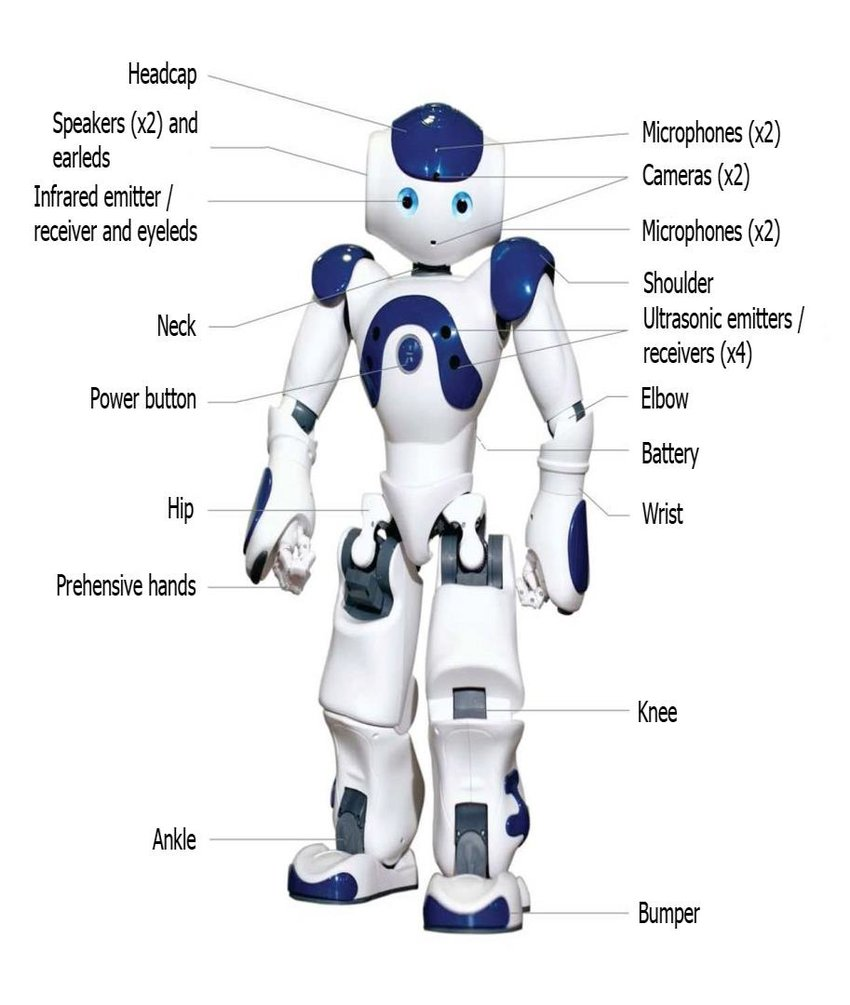
\includegraphics[width=0.45\textwidth]{nao}
    \caption*{Fonte: \cite{NAOxx}.}
    \label{fig:nao}
\end{figure}

\subsection{Robô DARWIN-OP}
\label{ssec:darwin}

O Darwin-OP (Dynamic Anthropomorphic Robot with Intelligence-Open Platform)  é um pequeno humanoide desenvolvido pela Robotis. Ele tem 20 graus de liberdade e pesa 2.9kg, possui uma camera HD, giroscópio, acelerômetro e um microfone stereo. O Darwin é capaz de andar, falar e dançar sendo bastante utilizado por pesquisadores e programadores.

\begin{figure} [H]
    \centering
    \caption{Robô Darwin-OP}
    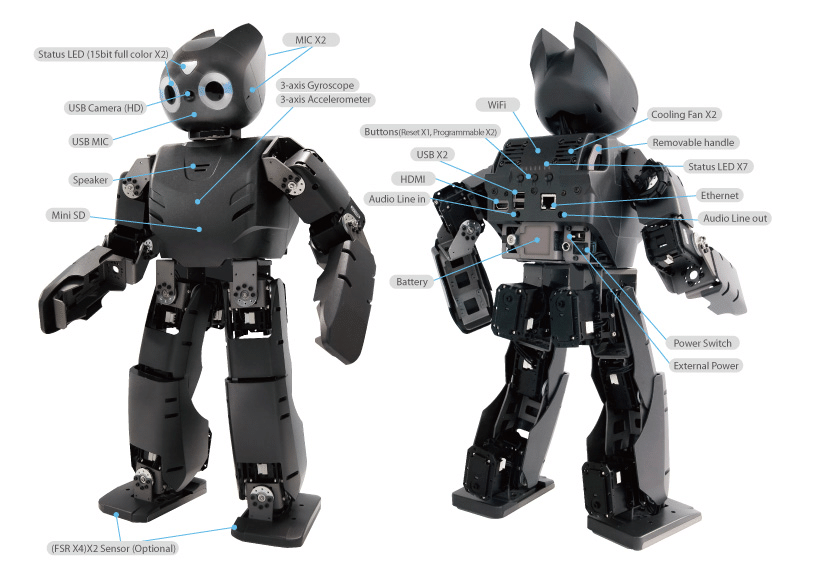
\includegraphics[width=0.65\textwidth]{darwin}
    \caption*{Fonte: \cite{DARWINxx}.}
    \label{fig:darwin}
\end{figure}

\subsection{Robô LOLA}
\label{ssec:lola}

O Lola é um robô humanoide desenvolvido na Universidade Técnica de Munich (TUM) e financiado pela Fundação de pesquisa alemã (DFG), utilizado em pesquisas sobre a dinâmica e aspectos de controle da locomoção bípede. A versão do Lola ilustrada na Figura \ref{fig:lola} possui 24 graus de liberdade, uma altura de 180cm e pesa aproximadamente 60kg. O seu design foi projetado para possuir pouco peso, uma rigidez efetiva alta, pernas com uma inércia baixa e o centro de gravidade alto. Com relação aos sensores utilizados pelo robô, o Lola possui enconders nos eixos dos seus motores e sensores de força/torque (FTS) customizados em seus pés, apresenta uma IMU em seu torso e uma câmera Intel RealSense em sua cabeça. É um robô versátil, com um design projetado para demonstrar uma caminhada bípede rápida.

\begin{figure} [H]
    \centering
    \caption{Robô LOLA}
    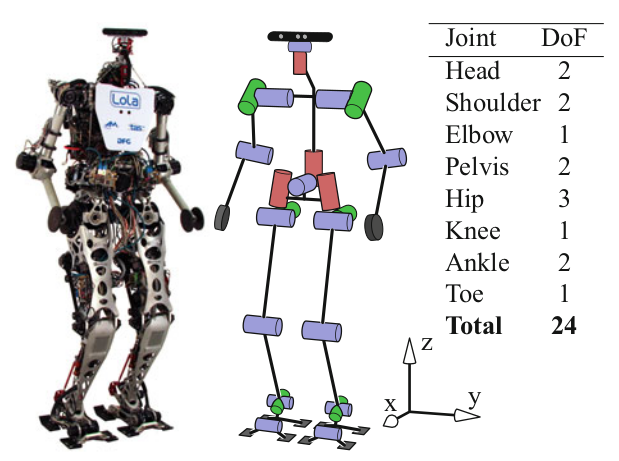
\includegraphics[width=0.6\textwidth]{lola}
    \caption*{Fonte: \cite{LOLAxx}.}
    \label{fig:lola}
\end{figure}

\subsection{Robô HUBO 2}
\label{ssec:hubo}

O HUBO 2 foi desenvolvido no laboratório HUBO no KAIST (Korean Advanced Institute os Science and Technology), na Coréia do Sul. Ele possui 125cm, pesa 45kg e possui 40 graus de liberdade. O seu design tinha como objetivo ser bem leve, o que permitiu que o HUBO 2 fosse capaz de correr em uma velocidade de 3.6 km/h. O seu sistema de percepção é composto por câmeras, sensores de inércia, inclinação e  força/torque. O seu grande diferencial em relação a outros robôs bípedes é a capacidade de utilizar uma marcha com pernas esticadas.

\begin{figure} [H]
    \centering
    \caption{Robô HUBO 2}
    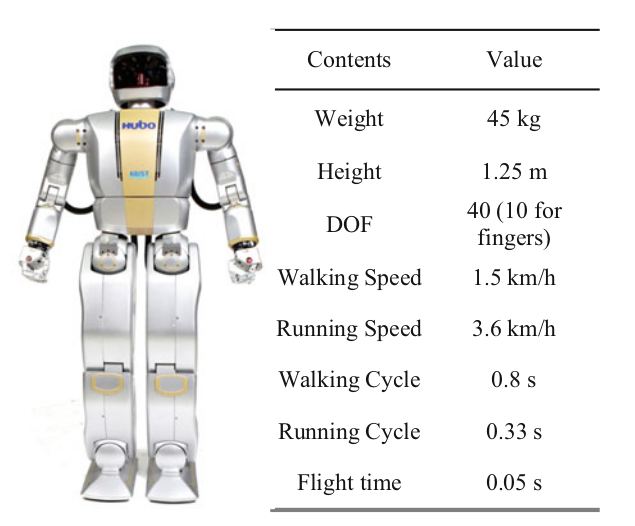
\includegraphics[width=0.5\textwidth]{hubo2}
    \caption*{Fonte: \cite{HUBOxx}.}
    \label{fig:hubo2}
\end{figure}


\section{Estudo das funcionalidades e mecânismos}
\label{sec:robos}

Nesta seção serão apresentadas as principais características dos sistemas de percepção e controle dos robôs antropormóficos, assim como da estrutura mecânica destes robôs. Estes são quesitos de extrema importância no desenvolvimento destes robôs pois influênciam na eficiência do seu sistema.

\subsection{Percepção}
\label{ssec:percepcao}

Os sensores comumente usados nos robôs humanoides podem ser classificados em dois grupos (Figura \ref{fig:sensors}), os sensores proprioceptivos são utilizados para medir os estados de cada junta e do corpo do robô e os sensores exteroceptivos são utilizados para obter informações do ambiente \cite{He2020}.

Os sensores internos são utilizados para medir o estado do robô, como ângulos, velocidades e torques das juntas. Para detectar informações da postura do robô, utiliza-se os sensores IMU, incluindo acelerômetros e giroscópios. Enquanto, a interação entre o robô e o ambiente podem ser detectadas por meio de sensores táteis e de força/torque. E, as câmeras e sensores de alcance medem e estimam as informações do ambiente ao redor do robô \cite{Ambarish20181}.

\begin{figure} [H]
    \centering
    \caption{Classificação dos sensores}
    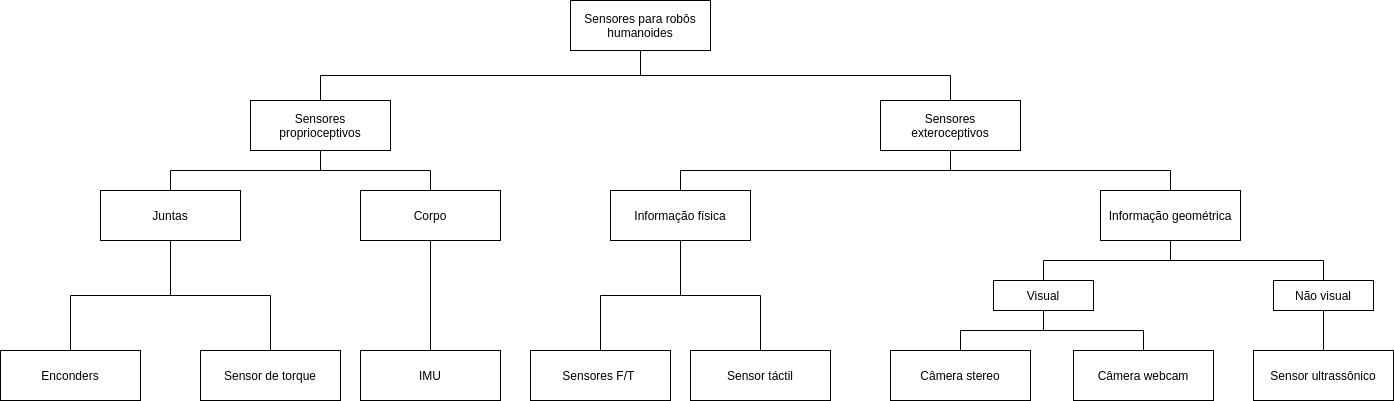
\includegraphics[width=\textwidth]{sensores}
    % \caption*{Fonte: Autoria própria.}
    \label{fig:sensors}
\end{figure}

O sistema de sensores do LOLA, por exemplo, de acordo com \citeonline{Buschmann2009141},  é otimizado para qualidade de sinal e largura de banda. Sensores angulares absolutos nos eixos de saída de todas as juntas compensam as elasticidades e não linearidades, permitindo que o robô (teoricamente) comece a partir de posições arbitrárias. Dois sensores de força / torque de seis eixos feitos sob medida são fortemente integrados à estrutura do pé. Com um peso total de 395g, o sensor inclui uma proteção contra sobrecarga. A unidade de medição inercial (IMU) estima a orientação e as velocidades angulares da parte superior do corpo. foi escolhida IMU de alta precisão com giroscópios de fibra ótica e acelerômetros MEMS, visto que a precisão e a qualidade do sinal do IMU afetam consideravelmente o desempenho do controlador de estabilização

%/todo: tabela com estes dados

Já no projeto desevolvido por \citeonline{Kien2017} quatro sensores ultrassônicos, dois em cada perna, são usados para feedback da posição para caminhar e girar. O acelerômetro é usado para medir o ângulo de inclinação e para detectar a queda instantânea do robô. Sensores Resistivos de Força (FSR) são usados para determinar o centro de pressão (COP), que por sua vez é usado para calcular o ZMP do robô.

%/todo: tabela com estes dados

\subsection{Mecânismos}
\label{ssec:mec}

Um robô humanoide tem o formato do corpo semelhante ao de um corpo humano e tem como base a literatura sobre a análise e coordenação da marcha humana. Eles possuem um grande número de graus de liberdade (DOF), para serem capazes de realizar um movimento bípede semelhante ao humano. Para que este movimento seja mais natural e flexível, segundo \citeonline{Buschmann2009141}, recomenda-se considerar uma configuração redundante com DOFs adicionais.

Para melhorar a dinâmica das pernas do robô deve-se garantir uma rigidez mecânica suficiente, centro de massa alto e baixos momentos de inércia dos elos das pernas.

O objetivo básico do projeto de um robô humanoide, é, portanto, equilibrar a rigidez estrutural e o desempenho do atuador com a leveza dos componentes mecânicos.
A estrutura mecânica do Lola, por exemplo, é caracterizado pelo design leve e consistente com alta rigidez efetiva \ref{ssec:lola}. São utilizados servo atuadores leves e a inércia resultante das pernas é minimizada por um design sofisticado da estrutura e mecanismos de acionamento, resultando em um comportamento de aceleração superior.

%/todo: abordar a estrutura de um robô menor
%/todo: inserir ilustrações

\subsection{Controle}
\label{ssec:control}

A figura \ref{fig:steps-control} ilustra os passos necessários para o controle da caminhada de um robô humanoide, onde a primeira etapa deste processo é o planejamento dos passos o qual é feito através do ajuste de alguns parâmetros de forma que o robô realize os movimentos de acordo com as fases de suporte dos pés ilustradas na figura \ref{fig:support-phases}.


\begin{figure} [H]
    \centering
    \caption{Elementos para o desenvolvimento do controlador de caminhada}
    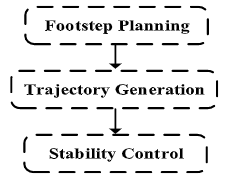
\includegraphics[width=0.3\textwidth]{walk-control}
    \caption*{Fonte: \cite{Kashyap2021306}.}
    \label{fig:steps-control}
\end{figure}


\begin{figure} [H]
    \centering
    \caption{Diferentes fases de suporte dos pés durante a locomoção de robôs humanoides}
    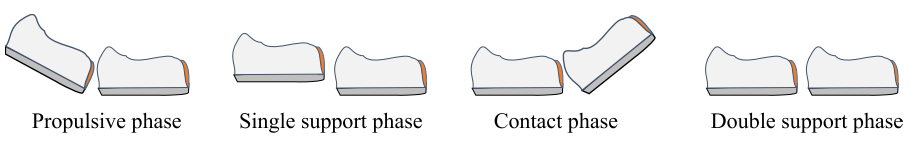
\includegraphics[width=0.8\textwidth]{support-phases}
    \caption*{Fonte: \cite{Kashyap2021306}.}
    \label{fig:support-phases}
\end{figure}

Existem basicamente dois tipos de marchas observadas em sistemas com pernas:  estaticamente estável e  dinâmicamente estável. Se o passo do robô permite que a projeção do seu centro de massa permaneça suficientemente dentro do polígono de suporte, projetado pelo pé do robô, então é estaticamente estável. E, se a projeção ocasionalmente sai do polígono de suporte , não deixando o robô cair ou tombar, então o sistema é dinâmicamente estável \cite{Ambarish20181}.

Existem quatro modelos que são frequentemente utilizados como representação aproximada do robô bípede (Figura \ref{fig:modelos-pendulos}). O Modelo do Pêndulo Invertido Linear (LIPM) considera que toda a massa do robô está concentrada em um ponto movendo-se em uma altura constante e assume que as pernas não possuem peso,  este modelo foi amplamente aplicado em diversas pesquisas como  por \citeonline{Kashyap2021306}, que utilizaram a técnica de optimização por enxame de partículas (PSO) para refinar o controlador PID convencional e bastante estudado e aplicado por \citeonline{Kajit201}.

\begin{figure} [H]
    \centering
    \caption{Modelos frequentemente utilizados como representações dos robôs bípedes}
    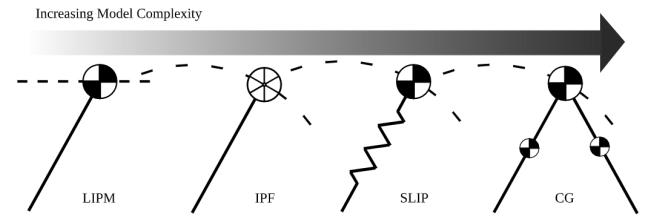
\includegraphics[width=0.8\textwidth]{modelos-pendulos}
    \caption*{Fonte: \cite{Grizzle20141955}.}
    \label{fig:modelos-pendulos}
\end{figure}

Um outro modelo é o Pêndulo Invertido com Volante (IPF) que não considera a altura constante e adiciona um volante para contabilizar o momento angular interno. O Pêndulo Invertido com Mola (SLIP) adiciona uma mola para modelar as pernas do robô como um pula-pula sem massa. E o Compass -Gait Biped (CG) que trata o robô como um pêndulo duplo com massas concentradas no centro de massa e nas pernas oscilantes \cite{Grizzle20141955}. Ao utilizar um modelo de robô reduzido \citeonline{Wahrmann20171471}, por exemplo, foi capaz de implementar a estratégia no controle em tempo real tornando o robô mais robusto contra erros de percepção e de superfícies irregulares. 

Posteriormente, deve-se implementar um gerador de trajetórias, o qual gera algum tipo de movimento considerando o deslocamento do Centro de Massa (COM) e do Ponto de Momento Zero (ZMP) assim como, a descrição da cinemática inversa. Desta forma, os ângulos das juntas do robô são obtidas. E, então é necessário um controlador para estabilizar estes ângulos  para garantir que o robô permaneça em pé e realize todas as tarefas sem cair. \cite{Kashyap2021306}

\citeonline{Kasaei2018743} apresenta uma estrutura de um controlador com um loop fechado baseada no método Central Pattern Generator (CPG) que propõem um modelo de controle inspirado nas características biológicas (Figura \ref{fig:arquitetura-nao}). Desta forma, este método tenta produzir um caminhar estável através de padrões rítmicos em relação a movimentação dos seus membros. Este teste foi realizado em um robô NAO simulado com a proposta de gerar uma movimentação estável e rápida.

\begin{figure} [H]
    \centering
    \caption{Arquitetura geral do gerador de passos}
    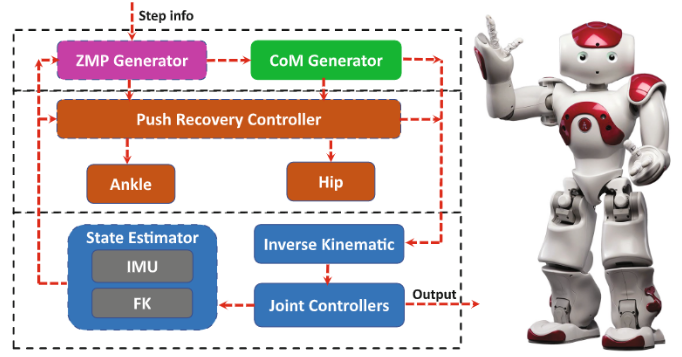
\includegraphics[width=0.4\textwidth]{arquiteturaNAO}
    \caption*{Fonte: \cite{Kasaei2018743}}
    \label{fig:arquitetura-nao}
\end{figure}

Em sua pesquisa \citeonline{Joe2019} implementam um framework de controle do equilíbrio que estabiliza os passos do robô em relação aos distúrbios. O controlador de equilíbrio é formado pelos controladores de orientação dos pés, comprimento da perna e ZMP. Os testes foram realizados no robô DRC-HUBO+ modificado. E, o framework proposto apresentou bons resultados permitindo que o robô se deslocasse de forma estável mantendo a postura desejada em terrenos irregulares.


\begin{figure} [H]
    \centering
    \caption{Visão geral do fluxo de informações do framework de controle de equilíbrio proposto}
    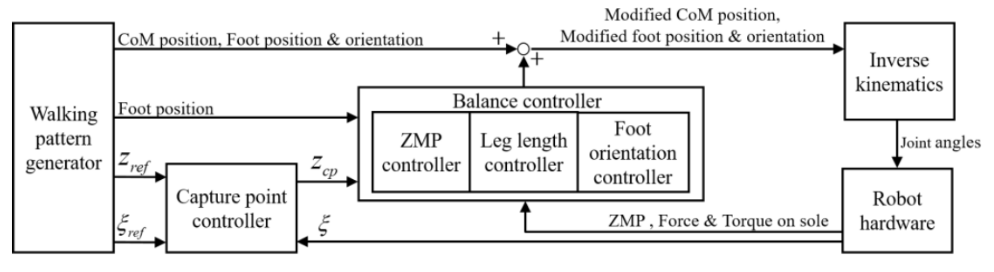
\includegraphics[width=0.8\textwidth]{controlador}
    \caption*{Fonte: \cite{Joe2019}}
    \label{fig:framework-control}
\end{figure}


O projeto de controle para sistemas subactuados são mais difícies devido a quantidade de graus de liberdades controláveis ser menor que a real quantidade de grau de liberdade do sistema. \citeonline{Gupta2017607} abordam outras estratégias de controle desenvolvidas para robôs subactuados como virtual constraints, HZD (Hybrid Zero Dynamics), Pointcaré map.



%******************************************************************

% \section{Mapa conceitual do estudo}
% \label{sec:mapa}



%******************************************************************

% \section{Organização e compartilhamento dos dados}
% \label{sec:org}


%******************************************************************






